\documentclass[12pt,a4paper]{article}
\usepackage[x11names]{xcolor}
\usepackage[T1]{fontenc}
\usepackage{xltxtra}
\usepackage{xunicode}

\usepackage[top=1.2in,bottom=1.2in,left=1.2in,right=1in]{geometry} % 页边距
\defaultfontfeatures{Mapping=tex-text}%连字号

\usepackage[boldfont,CJKchecksingle]{xeCJK} % 允许斜体和粗体
\xeCJKsetup{PunctStyle=hangmobanjiao}
\linespread{1.5} 							% 行间距
\setlength{\parskip}{\baselineskip} 	% 段间距
\usepackage{indentfirst}					% 首行缩进

\XeTeXlinebreaklocale "zh"
\XeTeXlinebreakskip = 0pt plus 1pt minus 0.1pt

\usepackage[unicode=true,colorlinks,linkcolor=blue]{hyperref} % 超链接
\setCJKmainfont[BoldFont=方正兰亭黑简体, ItalicFont=方正粗楷简体]{方正新书宋_GBK}
\setCJKsansfont[BoldFont=方正兰亭粗黑简体]{方正兰亭黑简体}
\setCJKmonofont[BoldFont=方正兰亭黑简体]{方正粗楷简体}
\setmainfont{Noto Serif}   					% 英文衬线字体
\setmonofont{DejaVu Sans Mono}   			% 英文等宽字体
\setsansfont{Noto Sans} 						% 英文无衬线字体

\usepackage{graphicx}        				% 嵌入png图像
\usepackage{longtable,tabu,booktabs}
\usepackage{pdflscape}

% specify width of included images
\LetLtxMacro{\OldIncludegraphics}{\includegraphics}
\renewcommand{\includegraphics}[2][]{~\\\OldIncludegraphics[width=0.9\textwidth, #1]{#2}}
\usepackage{tocloft} 							% 目录
\renewcommand\contentsname{目录}
\renewcommand{\today}{\number\year 年 \number\month 月 \number\day 日} % 中文日期

\begin{document}

\title{\textbf{StarRiver Server User Manual}}

\author{Pei Qing <qingpei@sansitech.com> \\
        Software Group, R\&D Dept.\\
        Shanghai Sansi Technology Co., Ltd.
}

\date{\vspace{3em} v1.0.0.3 \\\vspace{3em} \today}


\maketitle
\clearpage

\tableofcontents

\section{System Requirements}\label{system-requirements}

StarRiver Server and its database dependencies run on the following
hardware/software.

\subsection{Hardware}\label{hardware}

\begin{itemize}
\itemsep1pt\parskip0pt\parsep0pt
\item
  Minimum requirements

  \begin{itemize}
  \itemsep1pt\parskip0pt\parsep0pt
  \item
    Quad-core CPU. Intel Core i5 or higher.
  \item
    8GB RAM
  \item
    Fast Ethernet (100Mbps)
  \end{itemize}
\item
  Recommended setup

  \begin{itemize}
  \itemsep1pt\parskip0pt\parsep0pt
  \item
    Hexa-core CPU. Intel Xeon E5 or higher.
  \item
    32GB ECC RAM
  \item
    Gigabit Ethernet
  \end{itemize}
\end{itemize}

\begin{quote}
NOTE:Wired network is highly recommended. A wireless connection may
lead to high latency.
\end{quote}

\subsection{Software}\label{software}

\begin{itemize}
\itemsep1pt\parskip0pt\parsep0pt
\item
  Minimum

  \begin{itemize}
  \itemsep1pt\parskip0pt\parsep0pt
  \item
    Windows Server 2003
  \item
    MySQL Server 5.5 (MariaDB 5.5)
  \end{itemize}
\item
  Recommended

  \begin{itemize}
  \itemsep1pt\parskip0pt\parsep0pt
  \item
    Windows Server 2008 / Windows 7 or newer
  \item
    MySQL Server 5.6+ (MariaDB 10.0+)
  \end{itemize}
\end{itemize}

\begin{quote}
NOTE: As a Windows service, StarRiver Server can be remotely started /
stopped by our client application. This feature is not supported by
Windows XP.
\end{quote}

\section{安装服务器}\label{ux5b89ux88c5ux670dux52a1ux5668}

StarRiver 服务器的安装与配置分为两个部分:数据库和 StarRiver 通信程序。

\subsection{安装数据库}\label{ux5b89ux88c5ux6570ux636eux5e93}

StarRiver 采用 MySQL 或兼容 MySQL 的数据库系统(如 MariaDB)。下面以
MySQL Server 5.6 为例,介绍数据库的安装。

首先从\href{http://dev.mysql.com/downloads/mysql/}{MySQL
网站}下载安装程序。建议使用专门为 Windows 系统发布的 MySQL
Installer。本例中,我们采用
\href{http://dev.mysql.com/downloads/windows/installer/5.6.html}{MySQL
Installer 5.6.19} 版本。

安装步骤如下:

\begin{enumerate}
\def\labelenumi{\arabic{enumi}.}
\itemsep1pt\parskip0pt\parsep0pt
\item
  安装程序启动后是一个欢迎页面,我们选择「Install MySQL Products」。
  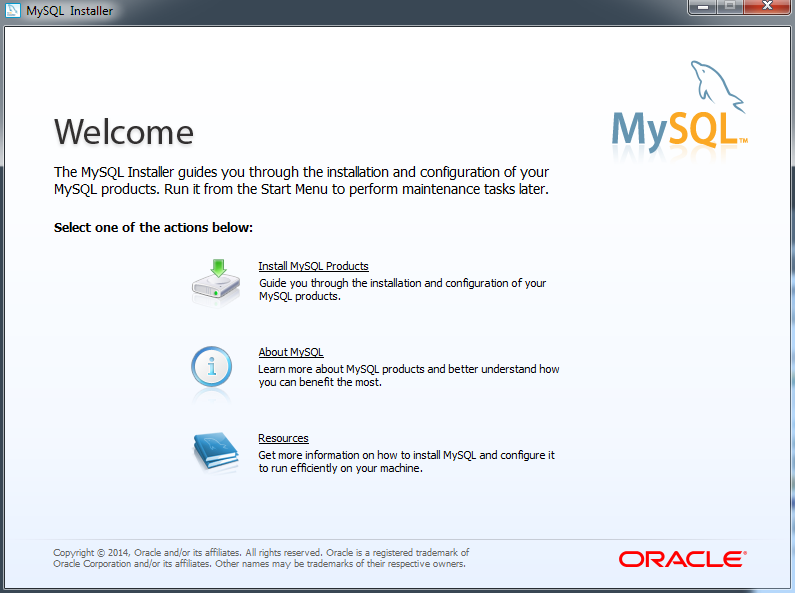
\includegraphics{img/mysql_1.png}
\item
  此时安装程序会尝试联网获取更新,如无 Internet 连接,可以勾选「Skip the
  check for updates」后继续。 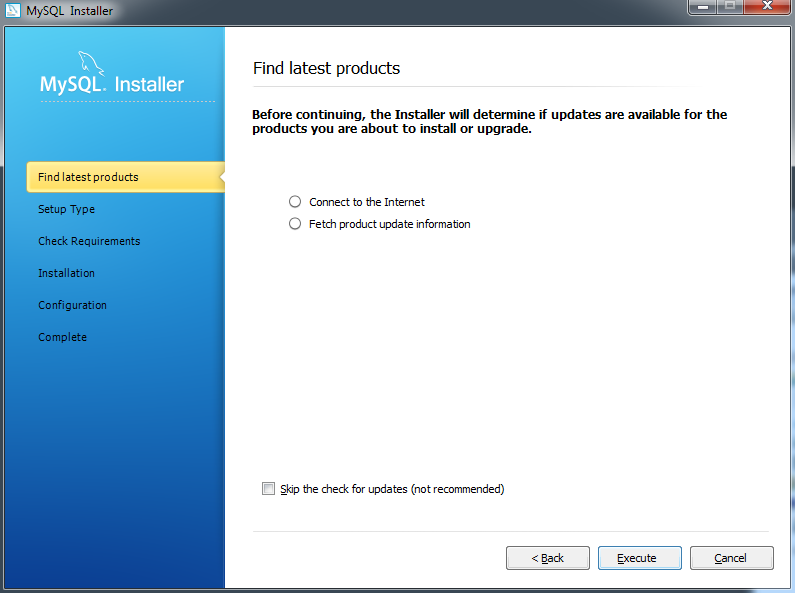
\includegraphics{img/mysql_2.png}
\item
  选择安装类型为「Server only」,并指定数据存放路径。此处我们以
  \texttt{C:\textbackslash{}MySQL\_Data}
  为例,您可以根据具体情况修改该路径。 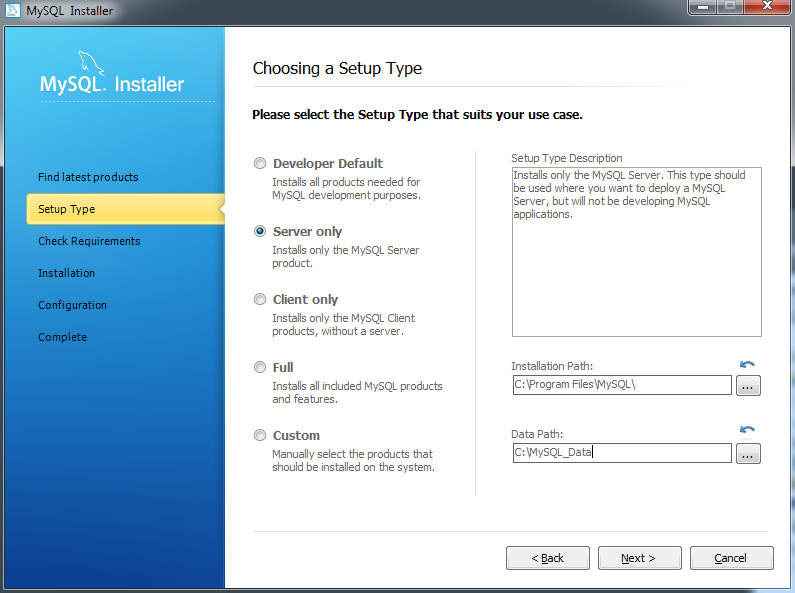
\includegraphics{img/mysql_3.png}
\item
  根据选择的安装项,安装程序检查是否有其他额外的依赖项目需要预先安装。如有,安装程序会下载安装;如无,则可以直接继续。
  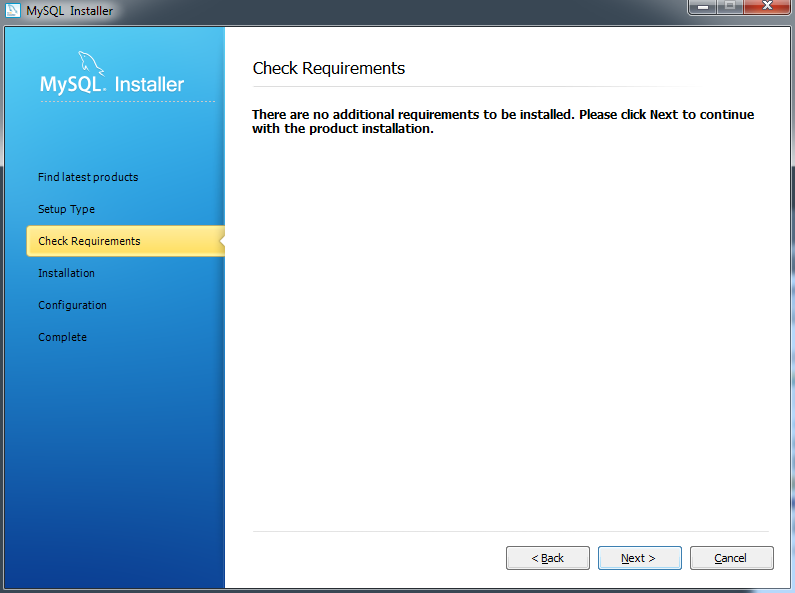
\includegraphics{img/mysql_4.png}
\item
  下面可以安装 MySQL Server 了。点击「Execute」开始安装。
  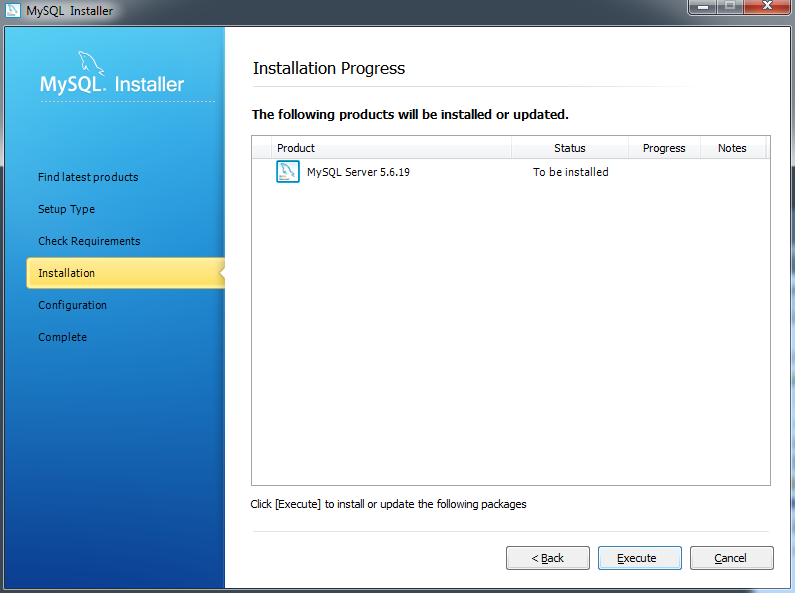
\includegraphics{img/mysql_5.png}
\item
  安装完成后可以进行初始配置,点击「Next」继续。
  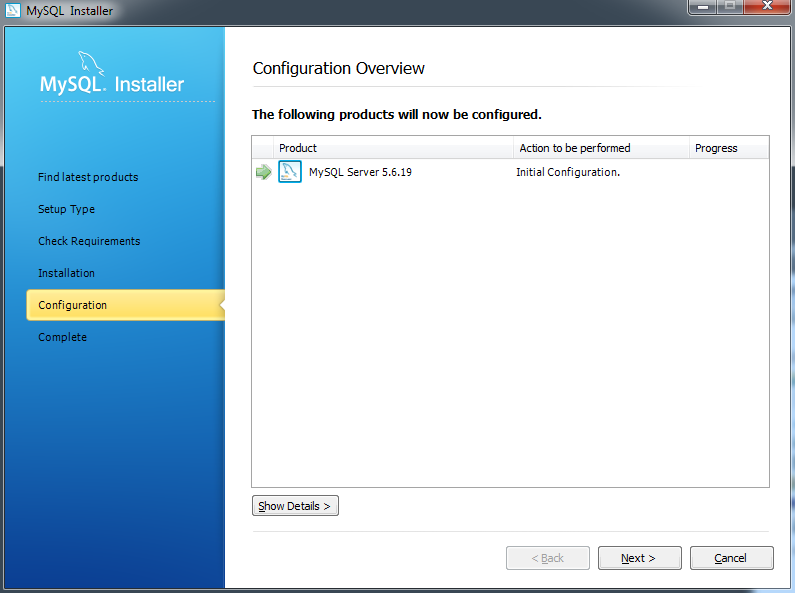
\includegraphics{img/mysql_6.png}
\item
  服务器配置类型选择「Server Machine」并继续。
  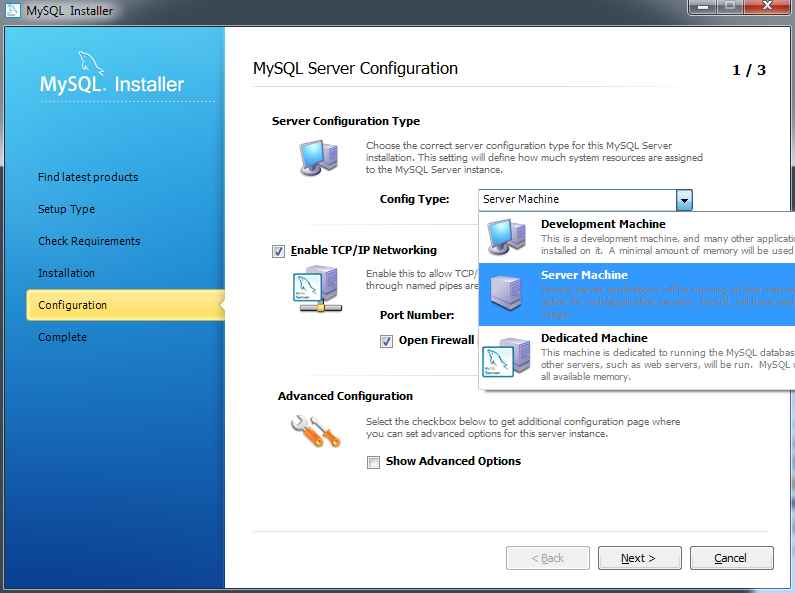
\includegraphics{img/mysql_7.png}
\item
  此处进行用户设置。设置 \texttt{root}
  用户的密码,建议设置复杂密码,并\textbf{请记住此处设置的密码}。单击「Add
  User」新建一个用户作为 StarRiver 的用户。用户名为
  \texttt{sansi},默认密码为
  \texttt{starriver}。\textbf{如您需要修改默认密码,请记住您设置的新密码,后续的配置需要用到这个密码。}
  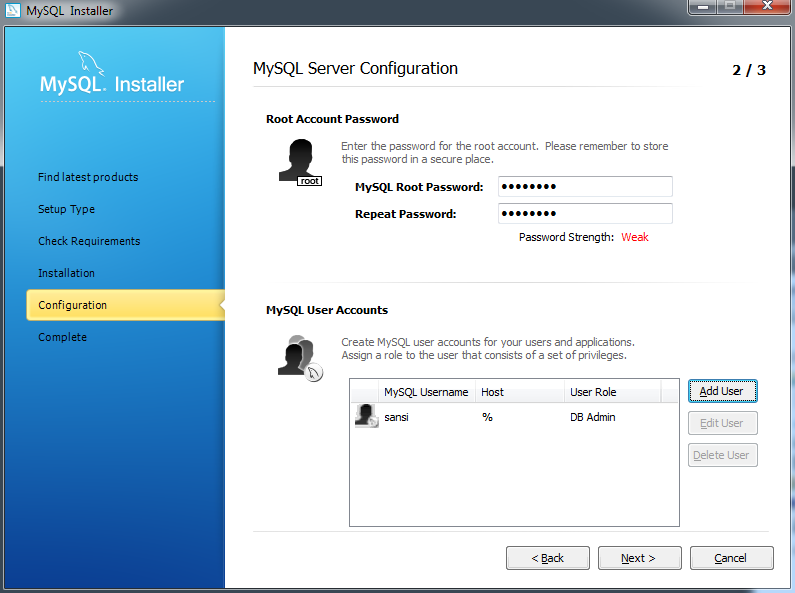
\includegraphics{img/mysql_8.png}
\item
  MySQL Server 将作为 Windows 服务启动,这里我们接受默认设置即可。
  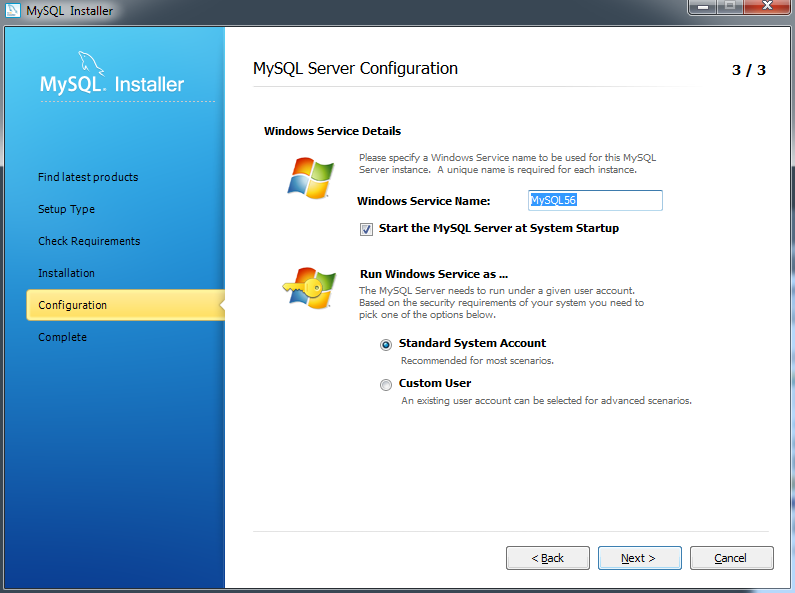
\includegraphics{img/mysql_9.png}
\item
  安装程序配置完成之后,点击「Next」继续。
  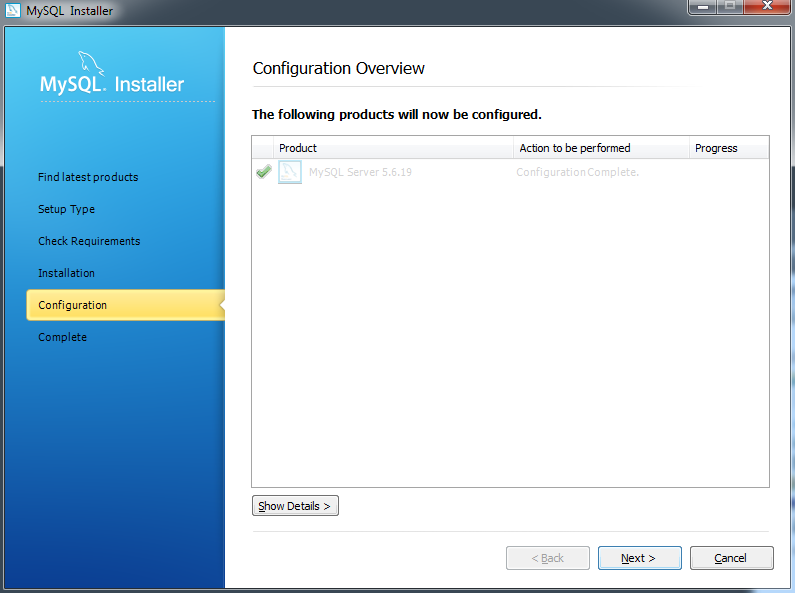
\includegraphics{img/mysql_10.png}
\item
  安装完成。 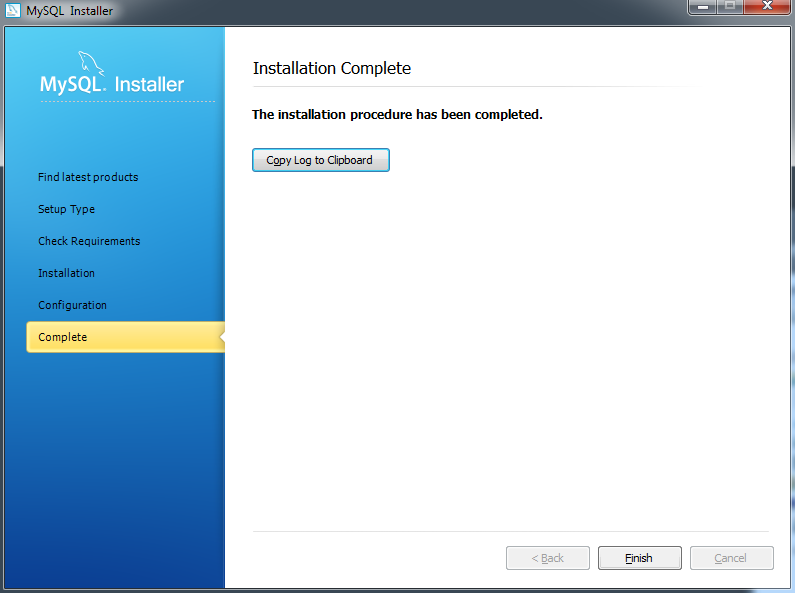
\includegraphics{img/mysql_11.png}
\end{enumerate}

接下来下载安装 \href{http://dev.mysql.com/downloads/workbench/}{MySQL
Workbench},方便我们管理数据库。此处我们采用 MySQL Workbench 6.1.7
版本。安装时全部接受默认选项即可。

最后在 MySQL Workbench 中,建立 StarRiver 需要的数据库表结构。

\begin{enumerate}
\def\labelenumi{\arabic{enumi}.}
\itemsep1pt\parskip0pt\parsep0pt
\item
  打开 MySQL Workbench,单击「MySQL
  Connections」右侧的「+」,新建一个服务器连接。
  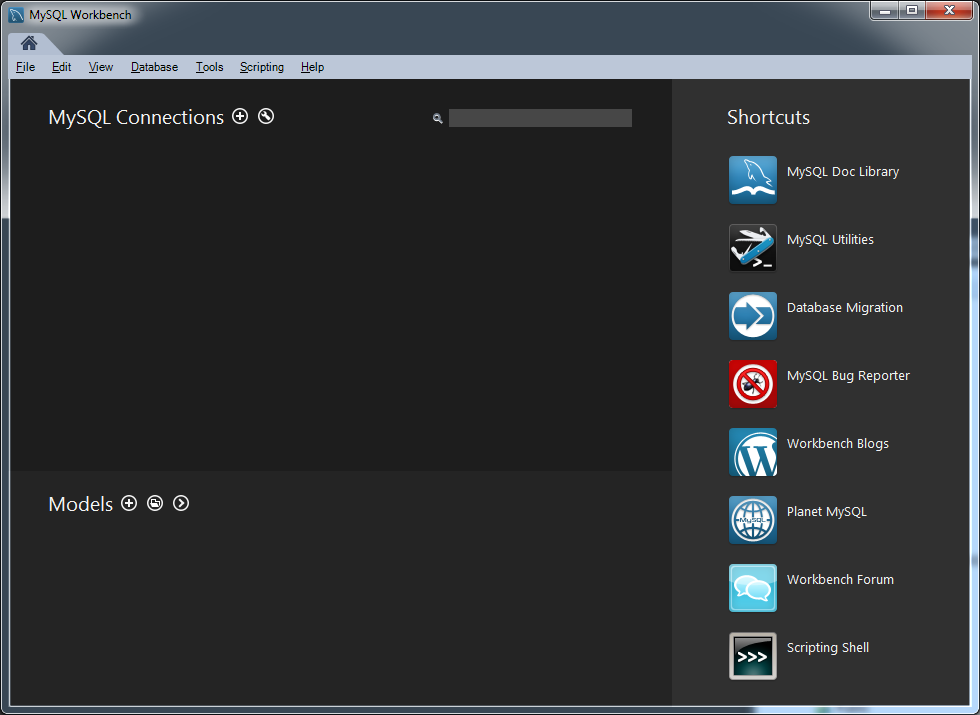
\includegraphics{img/db_init_1.png}
\item
  连接名为「StarRiver」,用户名为 \texttt{sansi},密码单击「Store in
  Vault \ldots{}」并输入 \texttt{starriver}。
  (如您在配置服务器建立用户时未使用默认密码,请输入您自定义的密码。)
  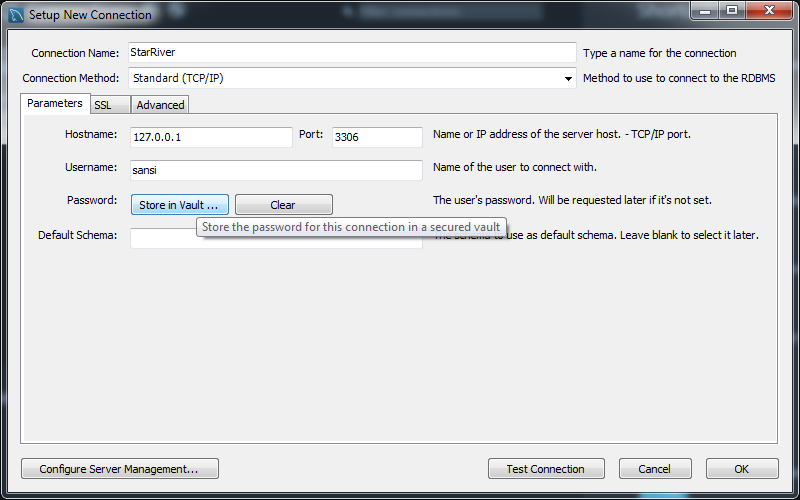
\includegraphics{img/db_init_2.png}
  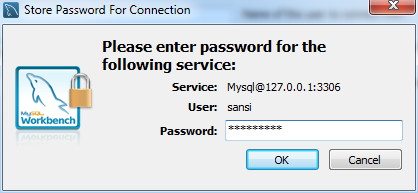
\includegraphics{img/db_init_3.png} 单击「Test
  Connection」,提示连接成功即可。如果报错则说明此前输入有误,请检查输入的用户名、密码等。
  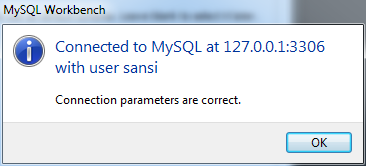
\includegraphics{img/db_init_4.png}
\item
  刚才新建的连接出现在界面上,单击它发起连接。
  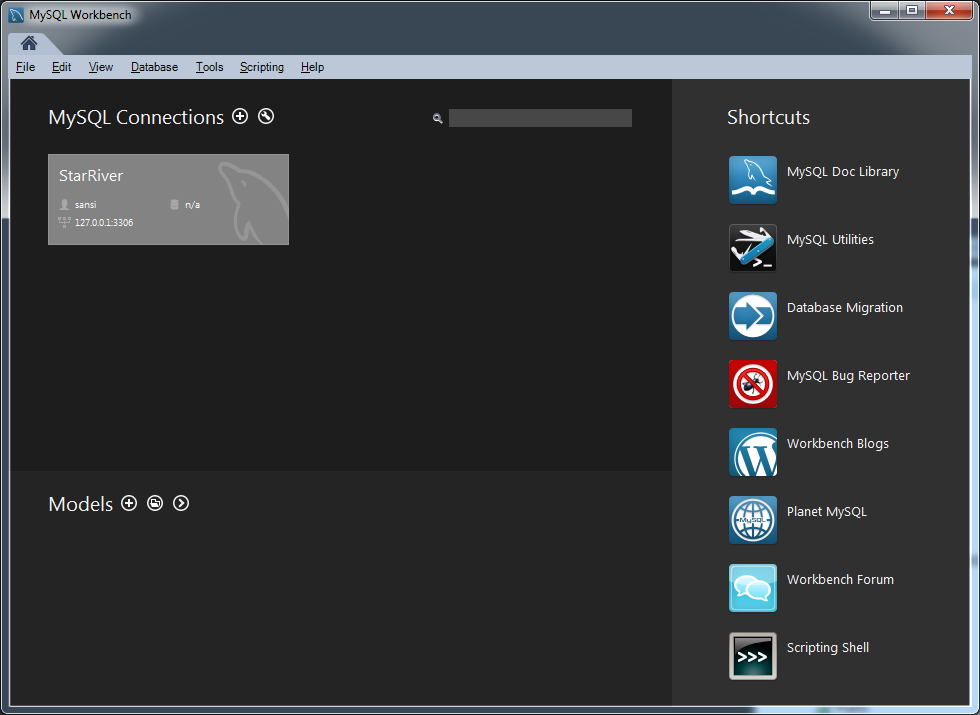
\includegraphics{img/db_init_5.png}
\item
  选择「File-\textgreater{}Open SQL Script」。
  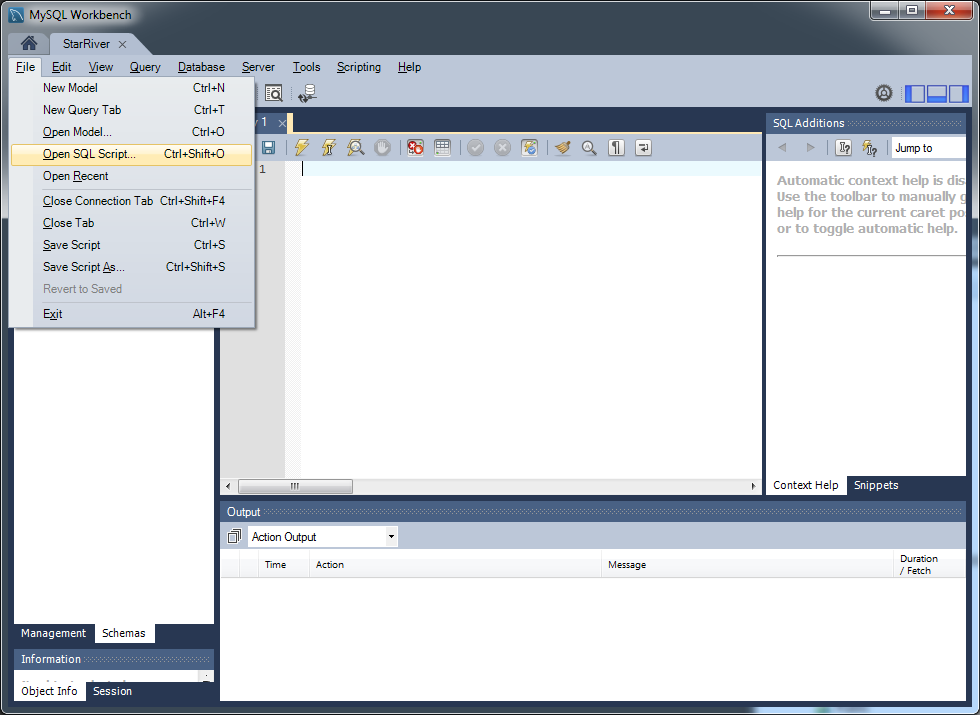
\includegraphics{img/db_init_6.png}
\item
  打开 \texttt{init\_schema.sql},单击图中框出的按钮执行脚本。
  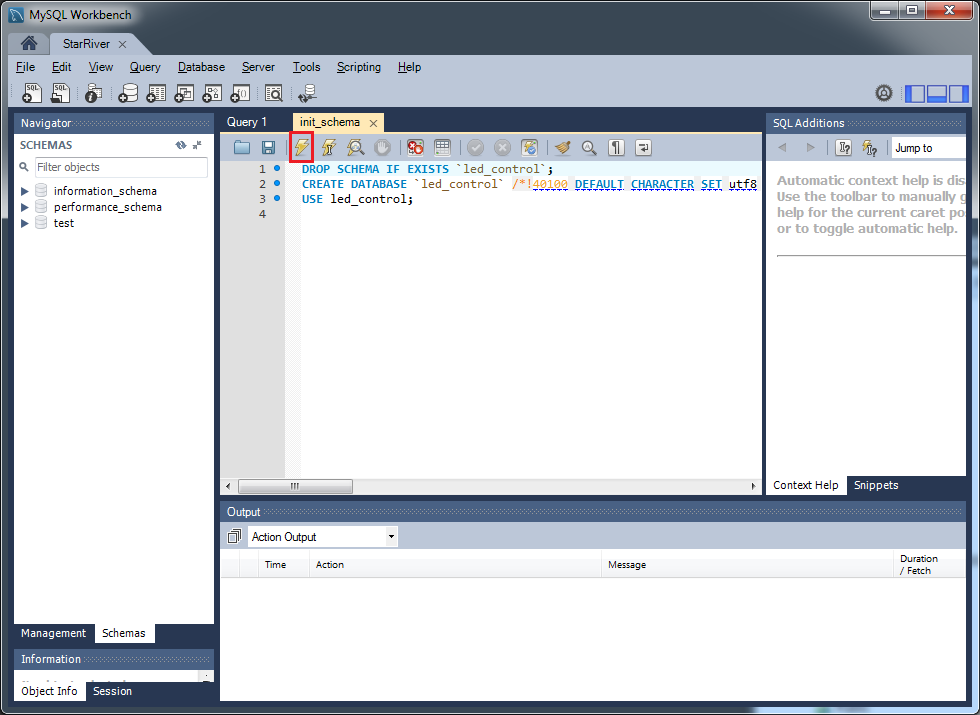
\includegraphics{img/db_init_7.png}
\item
  执行完毕,没有出错。 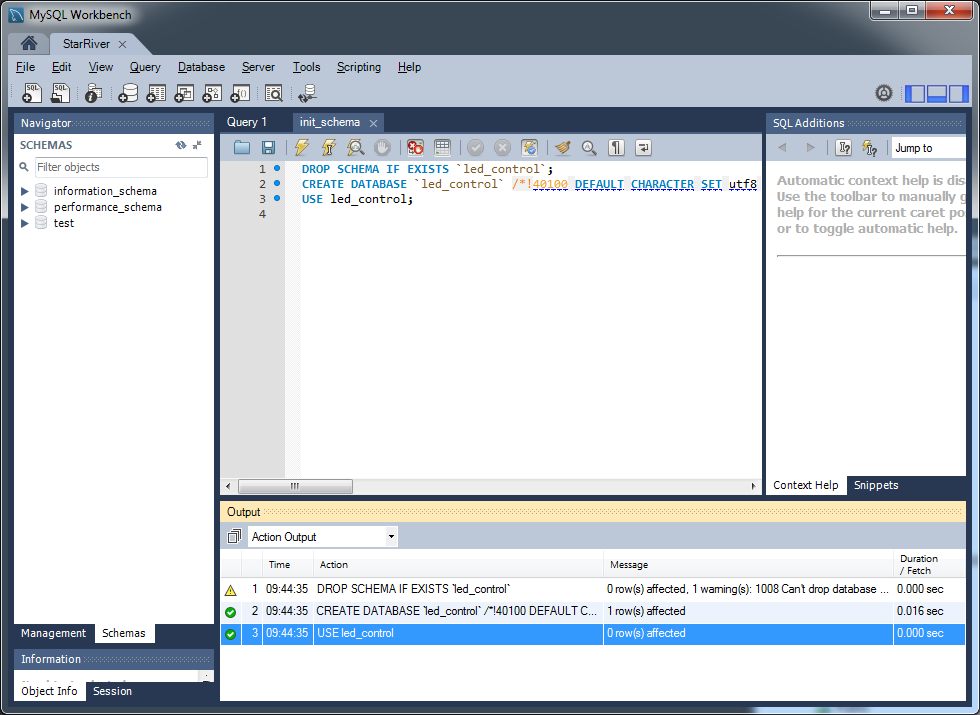
\includegraphics{img/db_init_8.png}
\item
  同样方式打开 \texttt{init\_db.sql},并执行。
  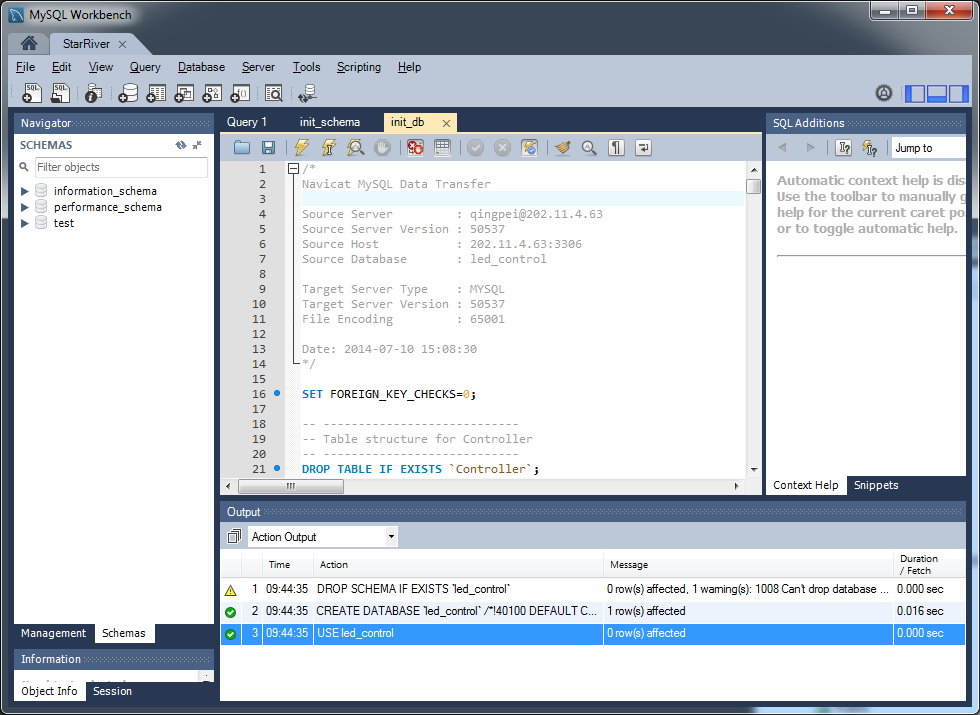
\includegraphics{img/db_init_9.png}
\item
  检查「Output」,没有出错。 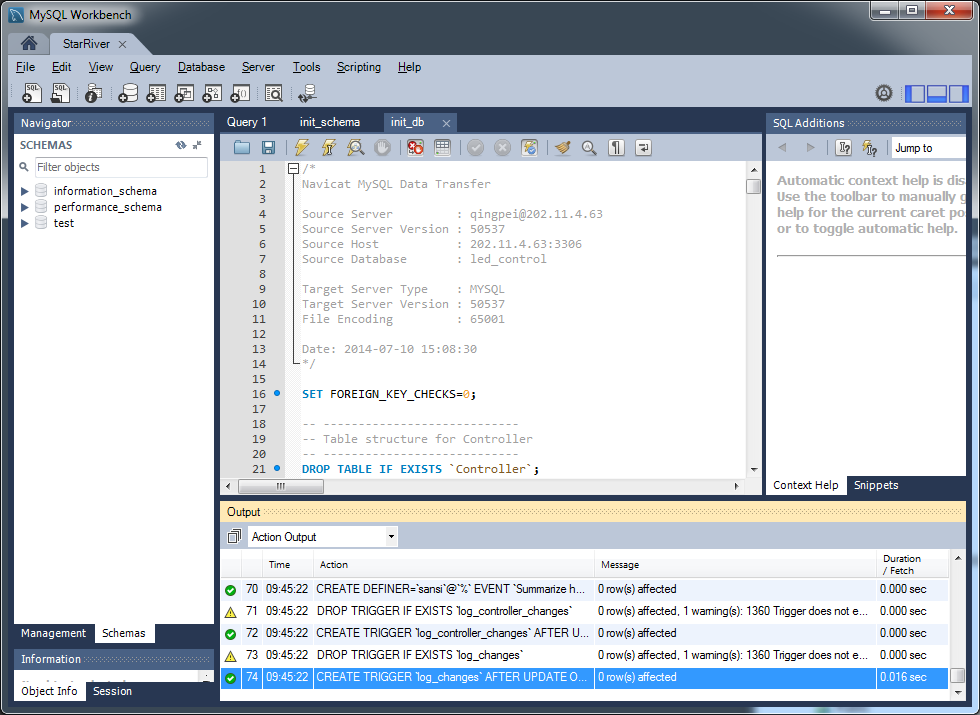
\includegraphics{img/db_init_10.png}
\item
  再打开 \texttt{init\_users.sql},并执行。
  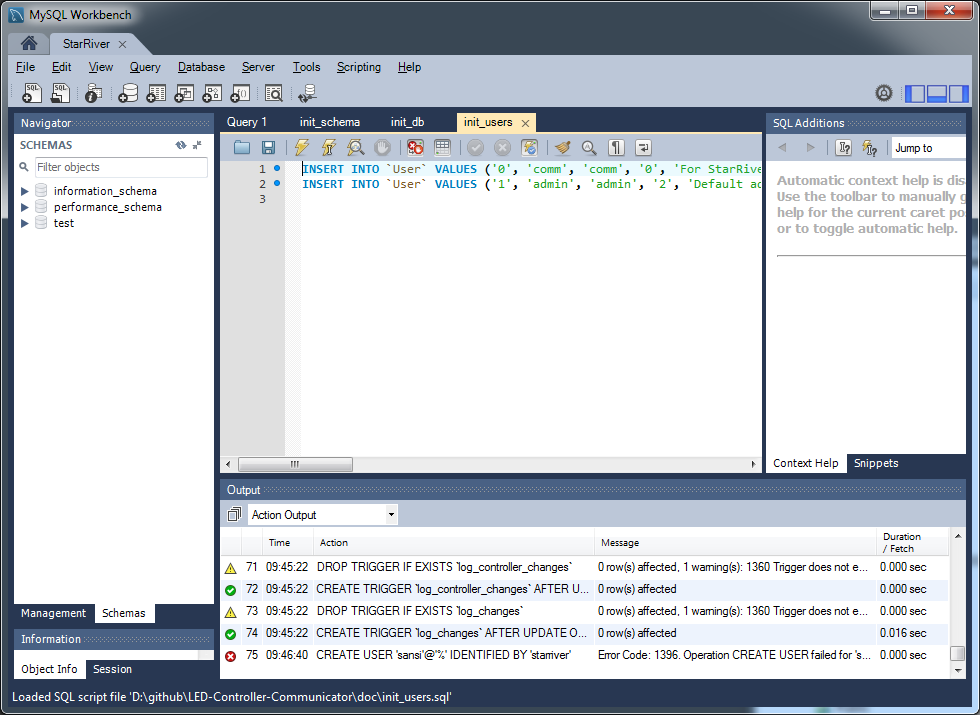
\includegraphics{img/db_init_11.png}
\item
  在左侧「Schemas」窗口内单击刷新按钮,看到名为 \texttt{led\_control}
  的数据库已经被成功建立。 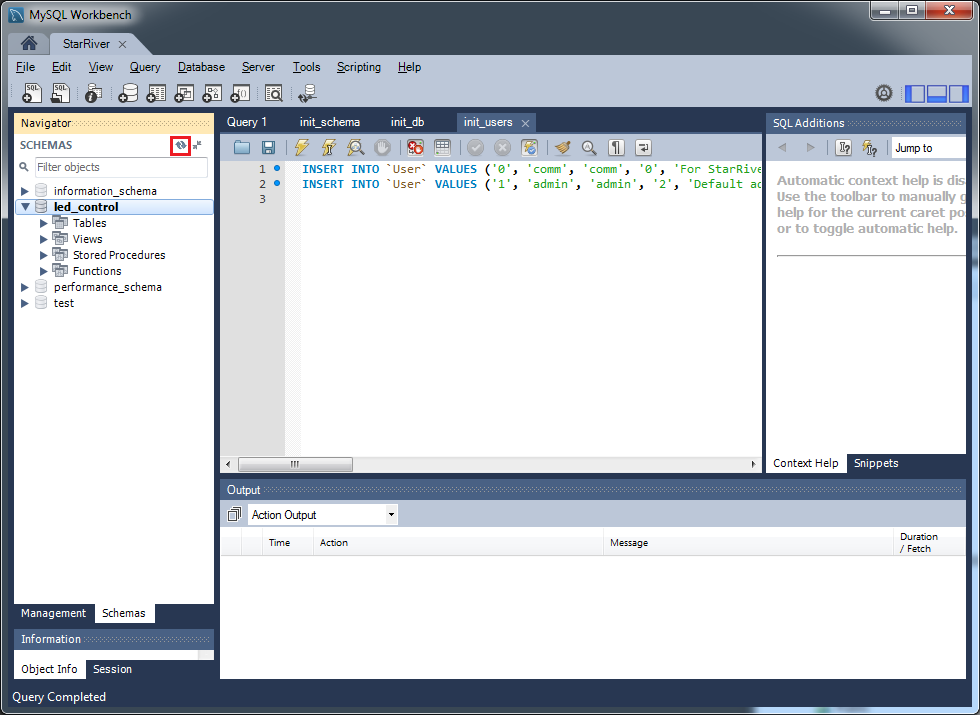
\includegraphics{img/db_init_12.png}
\end{enumerate}

\section{卸载服务器}\label{ux5378ux8f7dux670dux52a1ux5668}

\section{Start/Stop Server}\label{startstop-server}

StarRiver runs in background as a service. You could manually start or
stop the service via shortcuts in Start Menu.

\begin{figure}[htbp]
\centering
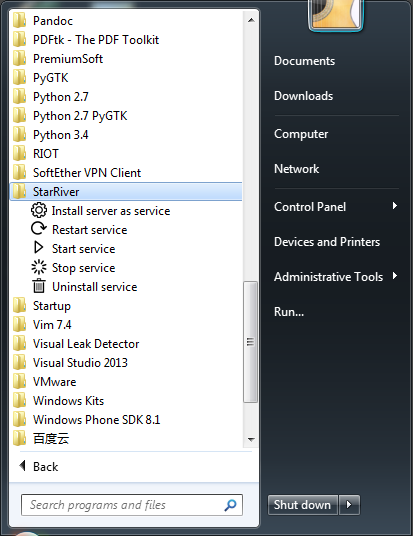
\includegraphics{../img/shortcuts.png}
\end{figure}

Five shortcuts created during installation are:

\begin{itemize}
\itemsep1pt\parskip0pt\parsep0pt
\item
  \textbf{Install server as service}: Install StarRiver Server as a
  Windows service. This has been done during installation.
\item
  \textbf{Restart service}: Manually restart StarRiver service.
\item
  \textbf{Start service}: Manually start StarRiver service.
\item
  \textbf{Stop service}: Manually stop StarRiver service.
\item
  \textbf{Uninstall service}: Remove the StarRiver Windows service.
  StarRiver communication application will not be removed. But it will
  no longer starts with the system.
\end{itemize}

\section{服务器日志}\label{ux670dux52a1ux5668ux65e5ux5fd7}

StarRiver 服务器运行时记录日志。日志存放在安装路径下,文件名格式为

\begin{verbatim}
LED_Control_Communicator_日期_时间.序号.log
\end{verbatim}



\end{document}
